%!TEX root = ..\arxiv_Dampinguncertanity_manuscript.tex
%-------------------------------
%*******************************
\section{BACKGROUND}
\label{sec:background}
%*******************************
We consider a single degree of freedom oscillatory system with viscous damping as
\begin{equation}
\ddot{x}+2 \xi \omega_{n} \dot{x}+\omega_{n}^{2} x=0,
\end{equation}
where $x$, $\dot{x}$ and $\ddot{x}$ are the oscillator displacement, velocity and acceleration respectively. $\xi$ is the damping ratio, $\omega_{n}$ is the natural frequency of the system.
The response of the system is given by
\begin{equation}
x(t)=A \mathrm{e}^{-\xi \omega_{n} t} \sin \left(\omega_{d} t+\varphi\right),
\end{equation}
where $\omega_{d}=\omega_{n} \sqrt{1-\xi^{2}}$, $A$ and $\varphi$ are determined by initial conditions.
From the logarithmic decrement method we know the damping ratio of a system with exponential decay is given by
\begin{equation}
\label{eqn1}
\xi=\frac{\delta}{\sqrt{\delta^{2}+4 \pi^{2}}},
\end{equation}
where $\delta=\frac{\ln \left(\frac{x_{0}}{x_{N}}\right)}{N}$ is the logarithmic decrement, $x_{0}$ is the magnitude of the first sample, and $x_{N}$ is the magnitude of the sample $N$ periods later.

Applying error propagation to Eq.~\ref{eqn1} gives the uncertainty in estimated damping $U(\xi)$ is related to uncertainty in the measurements $U_{x}$ by

\begin{equation}
\label{eq2}
U^{2}_{\xi}=\left[\left(\frac{\partial \xi}{\partial x_{0}}\right)^{2}+\left(\frac{\partial \xi}{\partial x_{N}}\right)^{2}\right] U_{x}^{2},
\end{equation}
evaluating Eq.~\ref{eq2} gives us

\begin{equation}
U^{2}_{\xi}=\frac{1}{4} \frac{\pi^{4}\left(-\xi^{2}+1\right)^{3}}{N^{2}\left(\pi^{2} \xi^{2}+\left(-\xi^{2}+1\right) \pi^{2}\right)^{3}}
\left( 1+\left(\frac{N \pi \zeta}{\mathrm{e}^{\sqrt{-\zeta^{2}+1}}}\right)^{2} \right) U_{x}^2.
\end{equation}
\begin{figure*}[h]



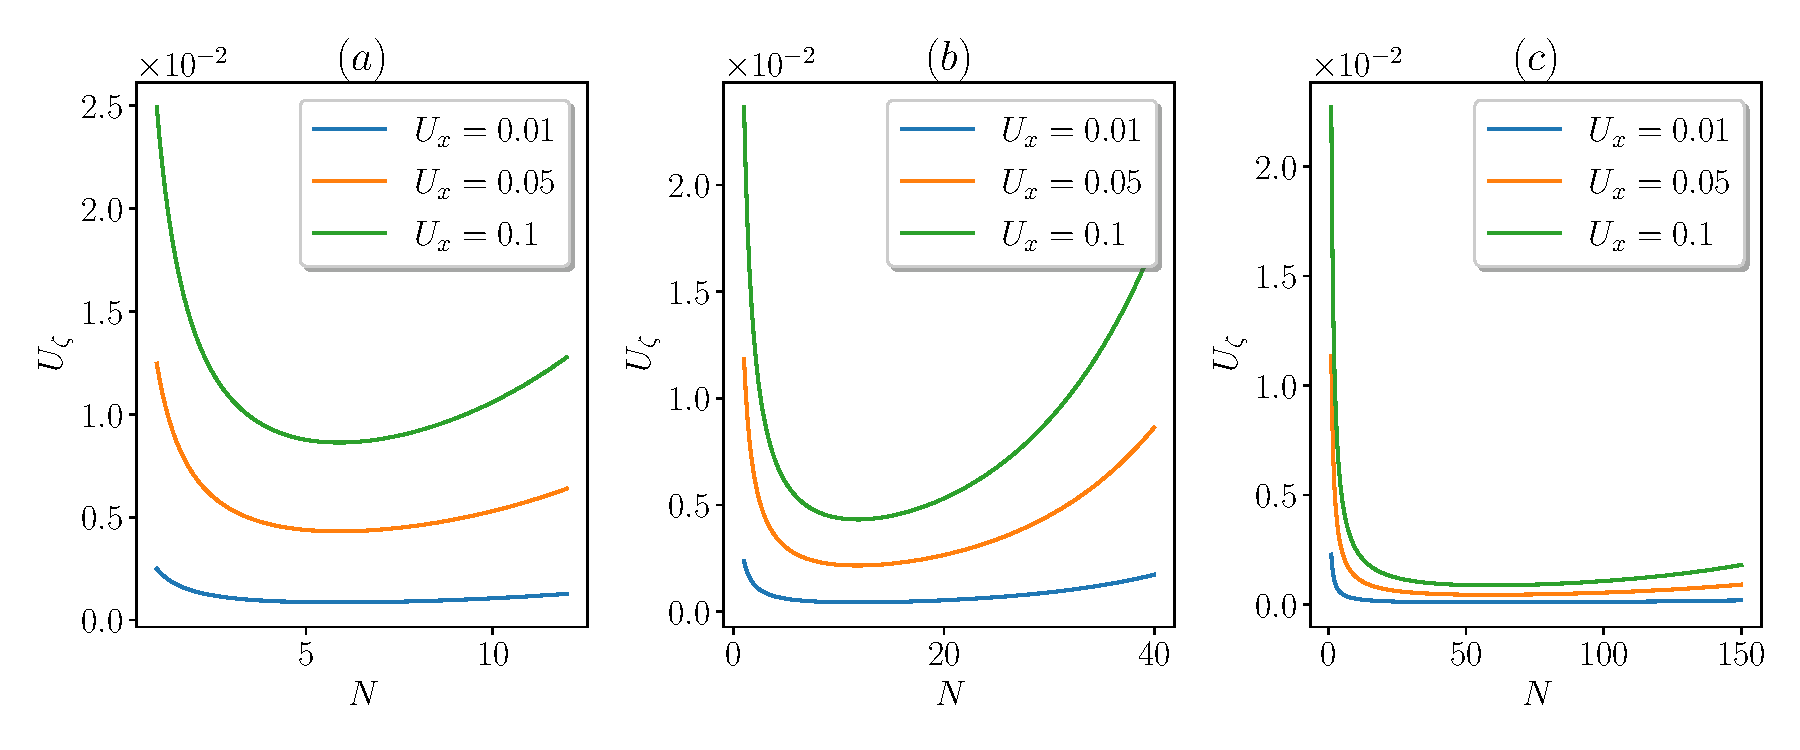
\includegraphics[scale=0.55]{fig1}
\centering
\caption{The variation of uncertainty $U_\xi$ with respect to  number of periods $N$ for various damping ratios($\xi$). (a) $\xi$ = 0.030, (b)$\xi$= 0.015, and (c)$\xi$ = 0.003.}
\label{f1}


\end{figure*}
Fig.~\ref{f1} shows the variation of uncertainty $U_\xi$ with respect to $N$ number of periods for various damping ratios($\xi$). (a) $\xi$ = 0.030, (b)$\xi$= 0.015, and (c)$\xi$ = 0.003.

 The optimal number of periods $N$ is obtained by differentiating $U_\xi$ with respect $N$ and solving for $N$, which is
\begin{figure}[h]


\centering

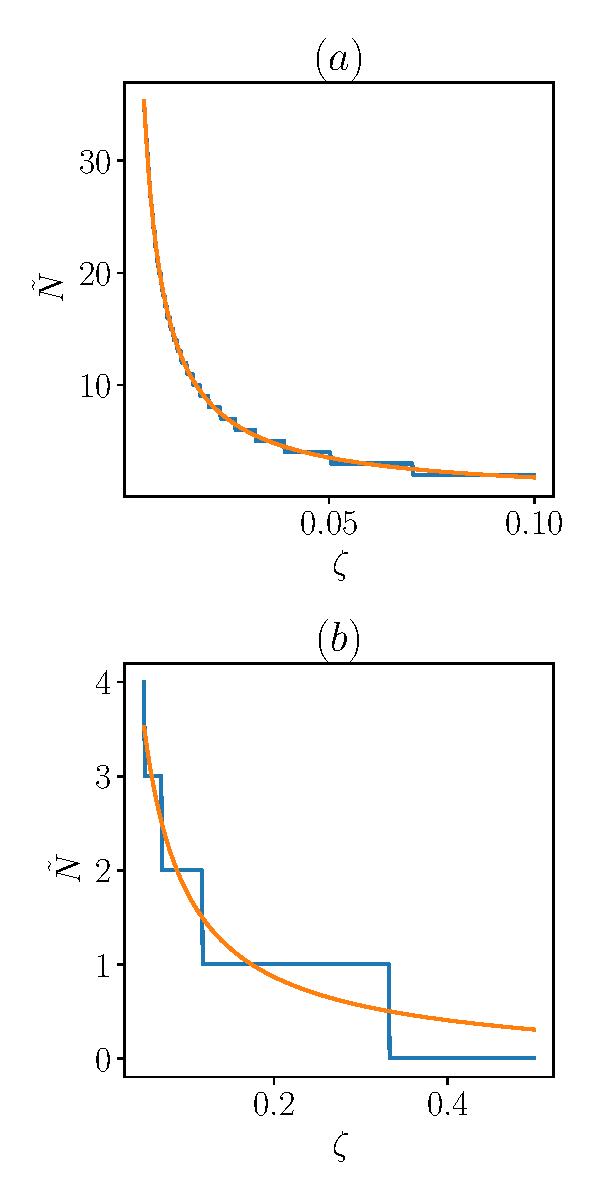
\includegraphics[scale=0.6]{fig3}
\caption{The optimal number of periods $N$ for predicting accurate damping ratios $\xi$ }
\label{f2}
\end{figure}

\begin{equation}
N_{\rm{opt}}=\frac{1}{4} \frac{\left(2+\mathrm{W}\left(2 \mathrm{e}^{-2}\right)\right) \sqrt{-(\xi-1)(\xi+1)}}{\pi \xi}.
\end{equation}
From Fig.~\ref{f2} we observe that uncertainty analysis gives us the optimum number of periods for damping ratios($\xi$) up to $0.1$. 
As the damping ratio increases beyond $0.1 $, we will be unable to determine the optimal number of periods.